\subsection{A graded intervention and converging controls}
\label{sec:graded}

Reflection is a large intervention, so we also move the bowl across seven registered lateral positions while retaining the same Nano checkpoint and 15 matched seeds per level (210 episodes). The requested-depth contrast changes gradually over the full support, with a slope of $1.12$\,m/m (95\% CI $[0.72,1.56]$); 13 of 15 seed-level slopes are positive (exact $p=.00739$). A post hoc middle-five sensitivity is weaker: $0.49$\,m/m (95\% CI $[-0.04,0.97]$), with 11 of 15 positive slopes ($p=.118$). We therefore claim a graded dependence across the registered seven positions, not an interior linear law. The fitted zero crossing lies outside the tested support.

\begin{figure*}[t]
  \centering
  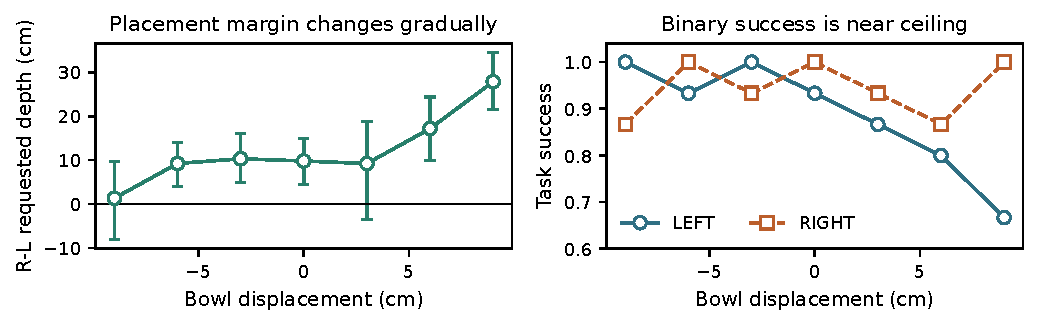
\includegraphics[width=0.98\textwidth]{figures/lateral_sweep.pdf}
  \caption{\textbf{The directional placement contrast changes across a seven-position reference-object sweep.}
  Left: mean RIGHT-minus-LEFT requested-side depth with seed-clustered 95\% intervals. Right: frozen task success by requested direction. Each position contains 15 matched seeds; the continuous measure exposes variation that binary success compresses near ceiling.}
  \label{fig:sweep}
\end{figure*}

Fig.~\ref{fig:sweep} also shows why binary success alone is a weak diagnostic here: LEFT completion changes from $15/15$ to $10/15$, while RIGHT stays close to ceiling. Separate interventions point in the same direction. Moving the target's start side changes success from $26/27$ versus $22/27$ to $23/27$ versus $27/27$ (interaction $+0.296$, $p=.0156$). Swapping target and reference roles changes the depth contrast by $+0.13$\,m (95\% CI $[0.06,0.21]$, $p=.00151$). Finally, 16 policy samples per fixed scene yield $41/216$ LEFT and $197/216$ RIGHT successes. The gap persists when policy sampling is repeated in these scenes; it is not an artifact of one draw.
